% !TEX program = pdflatex --shell-escape

\documentclass[11pt]{article}
\usepackage[round,sort&compress,semicolon]{natbib}
\usepackage{times}
\usepackage[T1]{fontenc}
\usepackage[utf8]{inputenc}
\usepackage[pdftex]{graphicx}\usepackage[letterpaper, left=1.0in, right=1.0in, top=1.0in, bottom=1.0in]{geometry}
\usepackage{ragged2e}
\usepackage{url}
\usepackage{setspace}
\usepackage{lineno}
\usepackage{multirow}
\usepackage{pdflscape}
\usepackage[backref=page]{hyperref}
\usepackage{rotating}
\usepackage{booktabs}
\usepackage[hypcap, labelsep=period, labelfont=bf]{caption}
\usepackage{array}
\usepackage{color}
\usepackage{soul}
\usepackage{mathtools}
\usepackage{pdflscape}

\usepackage{amsmath}
\usepackage{amsfonts}       % blackboard math symbols
\usepackage{nicefrac}       % compact symbols for 1/2, etc.
\usepackage{microtype}      % microtypography
\usepackage{doi}


\usepackage[dvipsnames,svgnames,table]{xcolor}
\urlstyle{same}
\setlength{\RaggedRightParindent}{\parindent}
\linenumbers
\linespread{1.1}

% restart counting in the supplement
\newcommand{\beginsupplement}{%
	\setcounter{table}{0}
	\setcounter{figure}{0}
	% \setcounter{section}{0}
	% \setcounter{subsection}{0}	
	\renewcommand{\thetable}{S\arabic{table}}%
	\renewcommand{\thefigure}{S\arabic{figure}}%
	% \renewcommand{\thesection}{S\arabic{section}}%
	% \renewcommand{\thesubsection}{S\arabic{section}.\arabic{subsection}}%          
}

%%% Add PDF metadata to help others organize their library
%%% Once the PDF is generated, you can check the metadata with
%%% $ pdfinfo template.pdf
\hypersetup{
     colorlinks   = true,
     citecolor    = Indigo,
     linkcolor    = DarkCyan,
}

\begin{document}

\begin{center}
	{\bf \Large
	% Redrawing the Boundaries of North American \emph{Delphinium}: Geography and Admixture 
	% Geography and Admixture Shape the Genome-Scale Phylogeny \\[0.2cm]
	% of North American \emph{Delphinium}
	% Towards a comprehensive phylogeny of North American \\
	% \emph{Delphinium} (Ranunculaceae)
	% Phylogenomic Evidence for Taxonomic Reevaluation in North American
	% \textit{Delphinium} and the Dominance of Geographic Patterns}\\[0.5cm]
	% Phylogenomic Evidence for a Major Taxonomic Revision of North American
	% \textit{Delphinium} and the Dominance of Geographic Patterns}\\[0.5cm]
	Geography and Admixture Shape the Genome-scale Phylogeny of \\
	North American \emph{Delphinium}\\[0.5cm]
	}

Jared B. Meek$^{1,*}$, Daniel Cook$^2$, B. Shaun Bushman$^3$, Deren A.R. Eaton$^{1,*}$\\[0.5cm]

1. Department of Ecology, Evolution, and Environmental Biology, Columbia University, 1200 Amsterdam Ave, New York, NY, 10027, USA;\\
2. USDA-ARS Poisonous Plant Research Laboratory, 1150 E 1400 N Logan, UT, 84341, USA;\\ 3. Forage \& Range Research Lab, Utah State University, Logan, UT 84322, USA;\\ 
* Corresponding Authors: jared.meek@columbia.edu; de2356@columbia.edu
% daniel.cook@usda.gov\\
% shaun.bushman@usda.gov\\

\end{center}

Keywords: Larkspur, Hybridization, Plant, Syngameon, Alpine, RAD-seq.

\RaggedRight

\section*{Abstract}

\section*{Introduction}
% Western North America contains unresolved plant clades that we need to understand better
North America is a topographically and ecologically complex region that has fostered the 
diversification of many endemic plant lineages. Its unique flora includes many rare and
specialized taxa narrowly distributed along climatic gradients, which now face mounting
threats from shifting climate and precipitation patterns, increased wildfire frequency, and habitat loss
\citep{kannenberg_rapid_2021,overpeck_climate_2020}.
% 
Although the region is among the most thoroughly studied botanical areas in the world
\citep{hickman1993jepson}, persistent taxonomic uncertainties hinder our ability to
accurately quantify biodiversity and track its decline. 
These knowledge gaps limit our ability to detect local extinctions \citep{wiens_climate-related_2016},
estimate species range shifts \citep{frei_plant_2010}, 
and scale ecological predictions across spatial hierarchies. 


The delimitation of species and their phylogenetic relationships remain poorly
understood even within some of the most enigmatic plant lineages of this region, 
such as larkspurs \citep[\emph{Delphinium};][]{jabbour_phylogeny_2012, xiang_recircumscription_2017} 
% penstemon
% louseworts \citep{yu_towards_2015}, 
beardtongues \citep[\emph{Penstemon};][]{wessinger_multiplexed_2016,wolfe_phylogenetics_2021},
and paintbrushes \citep[\emph{Castilleja}][]{tank_phylogenetic_2009,jacobs_quantifying_2019}.
% 
Such species-rich lineages often present taxonomic challenges owing to their 
rapid diversification and high frequency of hybridization.
% 
This is especially challenging for morphological systematics, where lineages
may be under- or over-split due to differences in rates of morphological evolution.
% 
Such patterns can be exacerbated in mountainous regions, where parallel adaptations
to similar environmental gradients cause cryptic variation, as in the case of 
\emph{Viburnum} in neotropical cloud forests \citep{donoghue_replicated_2022}. 
% 
When selection maintains distinct morphologies across environmental gradients, 
as in the case of desert \emph{Encelia} \citep{divittorio_natural_2020}, rare but 
distinct phenotypes that arise in hybrid populations can lead to inflated species 
descriptions.
% 
Systematic revisions that incorporate phylogenomic evidence can better
assess the distinctiveness of taxa by combining information from molecular
phylogenies, morphology, geography, and hybrid admixture 
\citep{hipp_genomic_2020}.
% 
This work contributes not only to improving plant taxonomy, but also to
our ability to quantify and preserve biodiversity; identify historical 
corridors of migration and dispersal; and investigate plant adaptations
to extreme conditions \citep{anstett_2021, gross_unforeseen_2024, melton_draft_2021}. 


A prime example of these dynamics is the North American clade of \emph{Delphinium} 
sect. \emph{Diedropetala} (Ranunculaceae), which has experienced a rapid radiation 
into approximtely 60 species since its arrival to western North America an 
estimated three million years ago \citep{jabbour_phylogeny_2012}.
% 
Species of this clade are perennial herbaceous plants characterized by large 
showy flowers that are typically blue and purple, and less commonly red, yellow, 
or white. 
% 
Many species are widespread and abundant in montane, grassland, and desert habitats,
while others exist as narrow endemics that have specialized adaptations to harsh 
alpine environments \citep{warnock_taxonomic_1995}. 
% 
Multiple species are currently endangered in North America. 
They are economically important as ornamentals, but are also intensely studied for 
their toxicity to livestock \citep{cook_biogeographical_2009, 
cook_two_2017, gardner_taxonomic_2002, pfister_grazing_2014}.
% Cook et al., 2009, 2017; Gardner et al., 2002; Pfister et al., 2014). 
Their rapid diversification in North America has been attributed to dispersal and 
isolation in the various mountain ranges of the western Cordillera, especially the
Cascades, Sierra Nevada, and Rocky Mountains \citep{warnock_taxonomic_1995}.
% 
Despite multiple taxonomic and phylogenetic research efforts focused on this clade,
there is no fully resolved phylogeny of \emph{Delphinium} sect. \emph{Diedropetala},
and little is known about its biogeographic history across western North America.


The genus \emph{Delphinium} is often considered taxonomically difficult due to a 
limited number of 
%distinguishable 
distinguishing
morphological characters. Two comprehensive 
taxonomic treatments for North American \emph{Delphinium} have been published over 
the last century which recognize between 60-80 species, but disagree over their
exact number, nomenclature, and distribution. 
% 
In the first published circumscription of the clade, Ewan \citep{ewan_synopsis_1945},
combined extensive 
fieldwork and study of herbarium specimens to distinguish 79 species grouped 
into 13 “series” based on seed morphology, leaf architecture and pubescence, 
corolla color, and other anatomical features. 
% 
Fifty years later, Warnock’s treatment \citep{warnock_taxonomic_1995}
reduced the number of species 
from 79 to 61, comprising two sections: \emph{Elatopsis}, represented by a garden 
cultivar (\emph{Delphinium elatum}) introduced from Europe, and 
\emph{Diedropetala}, which is composed of nine subsections.
%
These subsections are largely delineated by root structure and size, 
sepal color and length, seed morphology, and fruit position.
% 
This treatment is included in the current Flora of North America (FNA)
\citep{committee_flora_1997}, and we will refer to it hereafter as 
the FNA treatment.
Other notable taxonomic treatments in \emph{Delphinium} include:
\cite{rydberg_delphinium_1899, ewan_genus_1942, wilde1931studies, cronquist_intermountain_1984, ackerfield_flora_2022, chambers_comments_2018, lewis_taxonomic_1954,
koontz_delphinium_2012}.

In addition to these treatments, two molecular phylogenetic studies have used
Sanger sequencing markers to examine relationships within section \emph{Diedropetala}.
A study by \citet{koontz_using_2004} sampled sixty-two species of 
North American \emph{Delphinium} but found that few relationships can
be resolved using a small number of molecular markers. 
% 
A deeper-scale phylogenetic analysis by \cite{jabbour_phylogeny_2012} 
sampled a third of the North American species, as well as many other
species from across its global distribution.
Their results support section \emph{Diedropetala} as a monophyletic 
clade, but similarly lacked statistical power to confidently 
resolve many relationships within it.
% 
No study has yet brought genome-scale data to bear on phylogenetic 
relationships within \emph{Delphinium}.


% A paragraph about hybridization and the power of genomic data to resolve
Multi-locus phylogenomic analyses offer an advantage not only for inferring
species tree relationships from discordanct (conflicting) phylogenetic signals, 
but additionally for the potential to test for evidence of hybrid introgression
\citep{kubatko_species_2023}.
% 
Hybridization is likely to have played a significant role throughout the 
diversification of \emph{Delphinium}. 
Many putative hybrids have been described based on morphological descriptions 
\citep{ewan_synopsis_1945, warnock_taxonomic_1995, legro_species_1961, koontz_hybrid_2001},
but the extent to which they contribute to introgressive gene 
flow between species remains unknown.
% few have been confirmed using reproductive experiments or genomic 
% sequencing, 
% 
% EXPAND THIS SECTION A BIT>
% 
% Phylogenomic approaches that utilize thousands of loci have the power to distinguish hybrid introgression from neutral sources of discordance, such as incomplete lineage sorting, or a lack of phylogenetic information. 
In this study, we generated a new reduced-representation genomic dataset to 
investigate phylogeny and introgression across the \emph{Delphinium} sect. 
\emph{Diedropetala} clade. 
% 
We present a new and highly revised phylogenetic hypothesis for relationships
among species representing all previously described subsections in this clade 
% ({\bf Fig. 1}), 
and discuss our confidence in this result with regard to our 
extensive sampling of populations within species, tests for hybrid 
introgression, and the biogeographic concordance of our results.


%%%%%%%%%%%%%%%%%%%%%%%%%%%%%%%%%%%%%%%%%%%%%%%%%%%%%%%%%%%%%%%%%%%%%%%%%%%%%%%%%%%%%%%%%%%
%%%%%%%%%%%%%%%%%%%%%%%%%%%%%%%%%%%%%%%%%%%%%%%%%%%%%%%%%%%%%%%%%%%%%%%%%%%%%%%%%%%%%%%%%%%
%%%%%%%%%%%%%%%%%%%%%%%%%%%%%%%%%%%%%%%%%%%%%%%%%%%%%%%%%%%%%%%%%%%%%%%%%%%%%%%%%%%%%%%%%%%
%%%%%%%%%%%%%%%%%%%%%%%%%%%%%%%%%%%%%%%%%%%%%%%%%%%%%%%%%%%%%%%%%%%%%%%%%%%%%%%%%%%%%%%%%%%
\section{Materials and Methods}

\subsection{Taxon sampling}
We collected voucher specimens and silica-preserved leaf samples during field expeditions
between 2019-2022. Additional samples were provided by the USDA Poisonous Plant Research
Lab as part of a long-term research program concerning toxicity in \emph{Delphinium}, where
tissues were stored freeze-dried.
% 
This dataset includes 189 individuals, with replicate samples of 34 \emph{Delphinium} 
taxa collected from multiple geographically disjunct populations. Our sampling includes
at least one taxon as a representative of each subsection in the FNA treatment of
\emph{Delphinium}. 
We included samples from two \emph{Aconitum} species as outgroups.
All collections have associated geographic coordinates (Table S1) and voucher 
specimens available at the USDA Poisonous Plant Research Lab Herbarium (PPRL)
in Logan, UT.

\subsection{DNA sequencing and bioinformatics}
Genomic DNA was extracted from lyophilized leaf tissue using the Quick DNA
extraction kit (Zymo Research), adapted to a 96-well format. 
DNA quantity and quality were assessed using a spectrophotometer, TapeStation 
(Agilent), and gel electrophoresis, and genomic DNA was standardized to 20 ng/ul. 
% 
Genomic double-digest restriction-site associated DNA \citep[ddRAD-seq;][]{peterson_double_2012}
libraries were prepared at the USDA Forage \& Range Research Lab at 
Utah State University using the PstI and MspI restriction enzymes
\citep{poland_development_2012},
followed by adapter ligation, sample pooling, and a final purification
and partial polymerase chain reaction conducted for 16 cycles. 
% 
The pooled library was sequenced on an Illumina Nextseq 2000 at the Utah State 
University Center for Integrated Biosystems (Logan, UT) to produce single-end
75bp reads. 
% 
Sequence data for all samples was assembled in \emph{ipyrad} 
v.0.9.104 \citep{eaton_ipyrad_2020} using the \emph{de novo} 
pipeline and default parameter settings, except for the following
changes: datatype=ddrad, restriction\_overhang=(`TGCAG',`'),
filter\_adapters=2, maxdepth=10000, max\_SNPs\_locus=0.4,
max\_shared\_Hs\_locus=6, and max\_alleles\_consens=4. 
% 
% AFTER INFERRING A TREE?
% After running step 1 of \emph{ipyrad}, we subsampled the dataset to include
% at least three samples for each species distributed across multiple populations.
% This assembly, which consisted of 150 samples, excluded several misidentified
% samples and samples with fewer than 1,000 assembled consensus reads. 
% 
Additional downstream analyses 
%were performed in reproducible jupyter notebooks using 
used 
the \emph{ipyrad-analysis} toolkit to subsample and convert data to the
appropriate format for various analysis tools while also examining the impact of
missing data.
% We then ran steps 2-7 of ipyrad to create output files for downstream analyses,
% which were performed in reproducible jupyter notebooks using the 
% \emph{ipyrad-analysis} toolkit.

\subsection{Phylogenetic inference}
To investigate the impact of missing data on phylogenetic inference 
we generated supermatrices from all loci shared across at least four 
samples (`min4' dataset) or ten samples (`min10' dataset), using the
\emph{ipyrad-analysis} ‘window\_extracter’ tool \citep{eaton_ipyrad_2020}.
% 
For each dataset we inferred a maximum likelihood phylogenetic tree in
\emph{raxml-ng} v.1.2.2 \citep{kozlov_raxml-ng_2019} using the GTR+G substitution
model with four rate categories, starting from 10 random and 10 parsimony 
starting trees, and with 200 non-parametric bootstrap replicates. 
% 
Because concatenation can lead to biased inference in the presence of incomplete
lineage sorting, we also inferred a species tree from each dataset using 
\emph{caster} v.1.19 \citep{doi:10.1126/science.adk9688}, 
a quartet-based method that is consistent under the multispecies coalescent model. 
We used the `caster-site’ method which scores topologies for each site pattern 
shared among four taxa and infers a phylogeny by combining the quartet
trees with highest support. We used the settings --chunk 500 and --ambiguity 1. 
Support was assessed from 1000 local block bootstraps. 
The Python package \emph{toytree} \citep{eaton_toytree_2020} was used to 
visualize trees and compute tree distance metrics.

% A maximum-likelihood phylogenetic tree was inferred for the `min4’ and `min10’ datasets
% with \emph{raxml-ng} v.1.2.2 (Kozlov et al., 2019) using the GTR+G model with 4 rate 
% categories, starting from 10 random and 10 parsimony starting trees, and performing
% 200 non-parametric bootstrap replicates. Since concatenation can bias phylogenetic 
% inference in the presence of incomplete lineage sorting, we also inferred a species
% tree for our `min4’ dataset using CASTER v.1.19 (Zhang et al., 2025), a quartet-based
% method to infer a species tree from SNPs that is consistent under the
% multispecies coalescent model. We used the `caster-site’ model, which scores 
% topologies for each site pattern shared among four taxa and infers a phylogeny by 
% combining the quartet trees with highest support. Support was assessed from 
% 1000 local block bootstraps. Tree topologies compared using generalized 
% Robinson-Foulds distances calculated in the Python package \emph{toytree}
% \citep{eaton_toytree_2020}. 

To achieve a "population-level" phylogeny we additionally ran caster-site using 
a mapping file to assign individuals to populations. We included 41 
populations, where each represents a unique clade corresponding to a taxon name
that was consistently recovered as monophyletic in all phylogenetic analyses. 
Two clades did not meet this criterion.
We assigned the outgroup sample Acol2-3 to \emph{A. delphiniifolium} even though
it consistently groups with low support between the two outgroup clades. 
We assigned the sample Dalp4-2 to \emph{D. ramosum} population 4-10, 
since it consistently groups within that clade, despite being initially 
determined as \emph{D. alpestre}.
% and we lack sufficient confidence from only one sample to treat it
% as another \emph{D. alpestre} clade.
Caster-site was run using the same settings as above. 

%We then converted the branch lengths to obtain an ultrametric
%tree using penalized likelihood rate smoothing implemented in `toytree`,
%using four discrete rate categories, and with an external calibration on 
%the divergence time between \emph{Aconitum} and
%\emph{Delphinium} set to XX Ma, based on the previous analyses from 
%\citep{Jabbour}.

\subsection{Introgression analyses}
We calculated D-statistics \citep{durand_testing_2011} and F4-ratios using the
Dtrios method in Dsuite \citep{malinsky_dsuite_2021}, and plotted admixture 
proportions on species tree hypotheses using the f-branch statistic method.
This method requires a species tree hypothesis, and so we performed the test 
on three trees, using the population-level tree inferred by caster-site, 
as well as population-level trees matching the ML min4 and min10 topologies, 
created by similarly collapsing monophyletic clades into a single tip.
Analyses were run using a VCF file from the min10 assembly, and with the 
parameter -k 500 to set the number of jackknife blocks.
% 
For all tests we used the pooled allele frequencies among the outgroup samples 
of \emph{Aconitum} as the P4 taxon. We also used allele frequencies among pooled
replicate samples from monophyletic species, or populations, to represent the
P1, P2, or P3 taxa. 
% 


\subsection{Investigating hybrid complexes}
To investigate non-monophyletic taxon relationships in a complex formed 
by \emph{D. robustum}, \emph{D. ramosum}, and \emph{D. alpestre}, 
we performed additional phylogenetic and principal component analyses.
% 
We used the ipyrad-analysis window-extracter tool to extract a sequence 
alignment that includes data only for taxa in the subclade (18 samples), 
in addition to two outgroup taxa. 
Here we used \emph{D. californicum} and \emph{D. hesperium} as more closely 
related outgroups than \emph{Aconitum}, since these taxa showed no evidence
of admixture with other taxa, and are suitable to serve as outgroups for this analysis.
% 
These alignments include all sites with data shared across at least 10 
samples (min10), and were input to raxml-ng with the same settings described
above to infer ML trees. 
% 
To examine population structure we used the ipyrad-analysis pca tool to 
extract unlinked SNPs and perform Principal Component Analyses (PCA). 
% 
We ran this analysis on both the focused dataset (18 samples) and on a
larger dataset that includes other closely related species and potentially
admixed species (39 samples).
% 
For each analysis we retained only bi-allelic SNPs with zero missing data across
the subset of samples examined, and randomly subsampled one SNP per RAD locus to
reduce the effect of linkage. 
% 
To examine variation over the randomly sampled subset of unlinked SNPs we 
performed 50 replicate analyses and plotted the centroid point for each sample
over a low-opacity cloud of points from all replicates.
% 
Results were contextualized relative to the geographic distribution of 
samples examined in interactive Folium maps generated with the 
Esri.WorldTopoMap base layer (Sources: Esri, HERE, Garmin, Intermap, 
INCREMENT P, GEBCO, USGS, FAO, NPS, NRCAN, GeoBase, IGN, Kadaster NL, 
Ordnance Survey, Esri Japan, METI, Esri China (Hong Kong), © OpenStreetMap 
contributors, GIS User Community).


\begin{figure}[t!]
	\centering
	  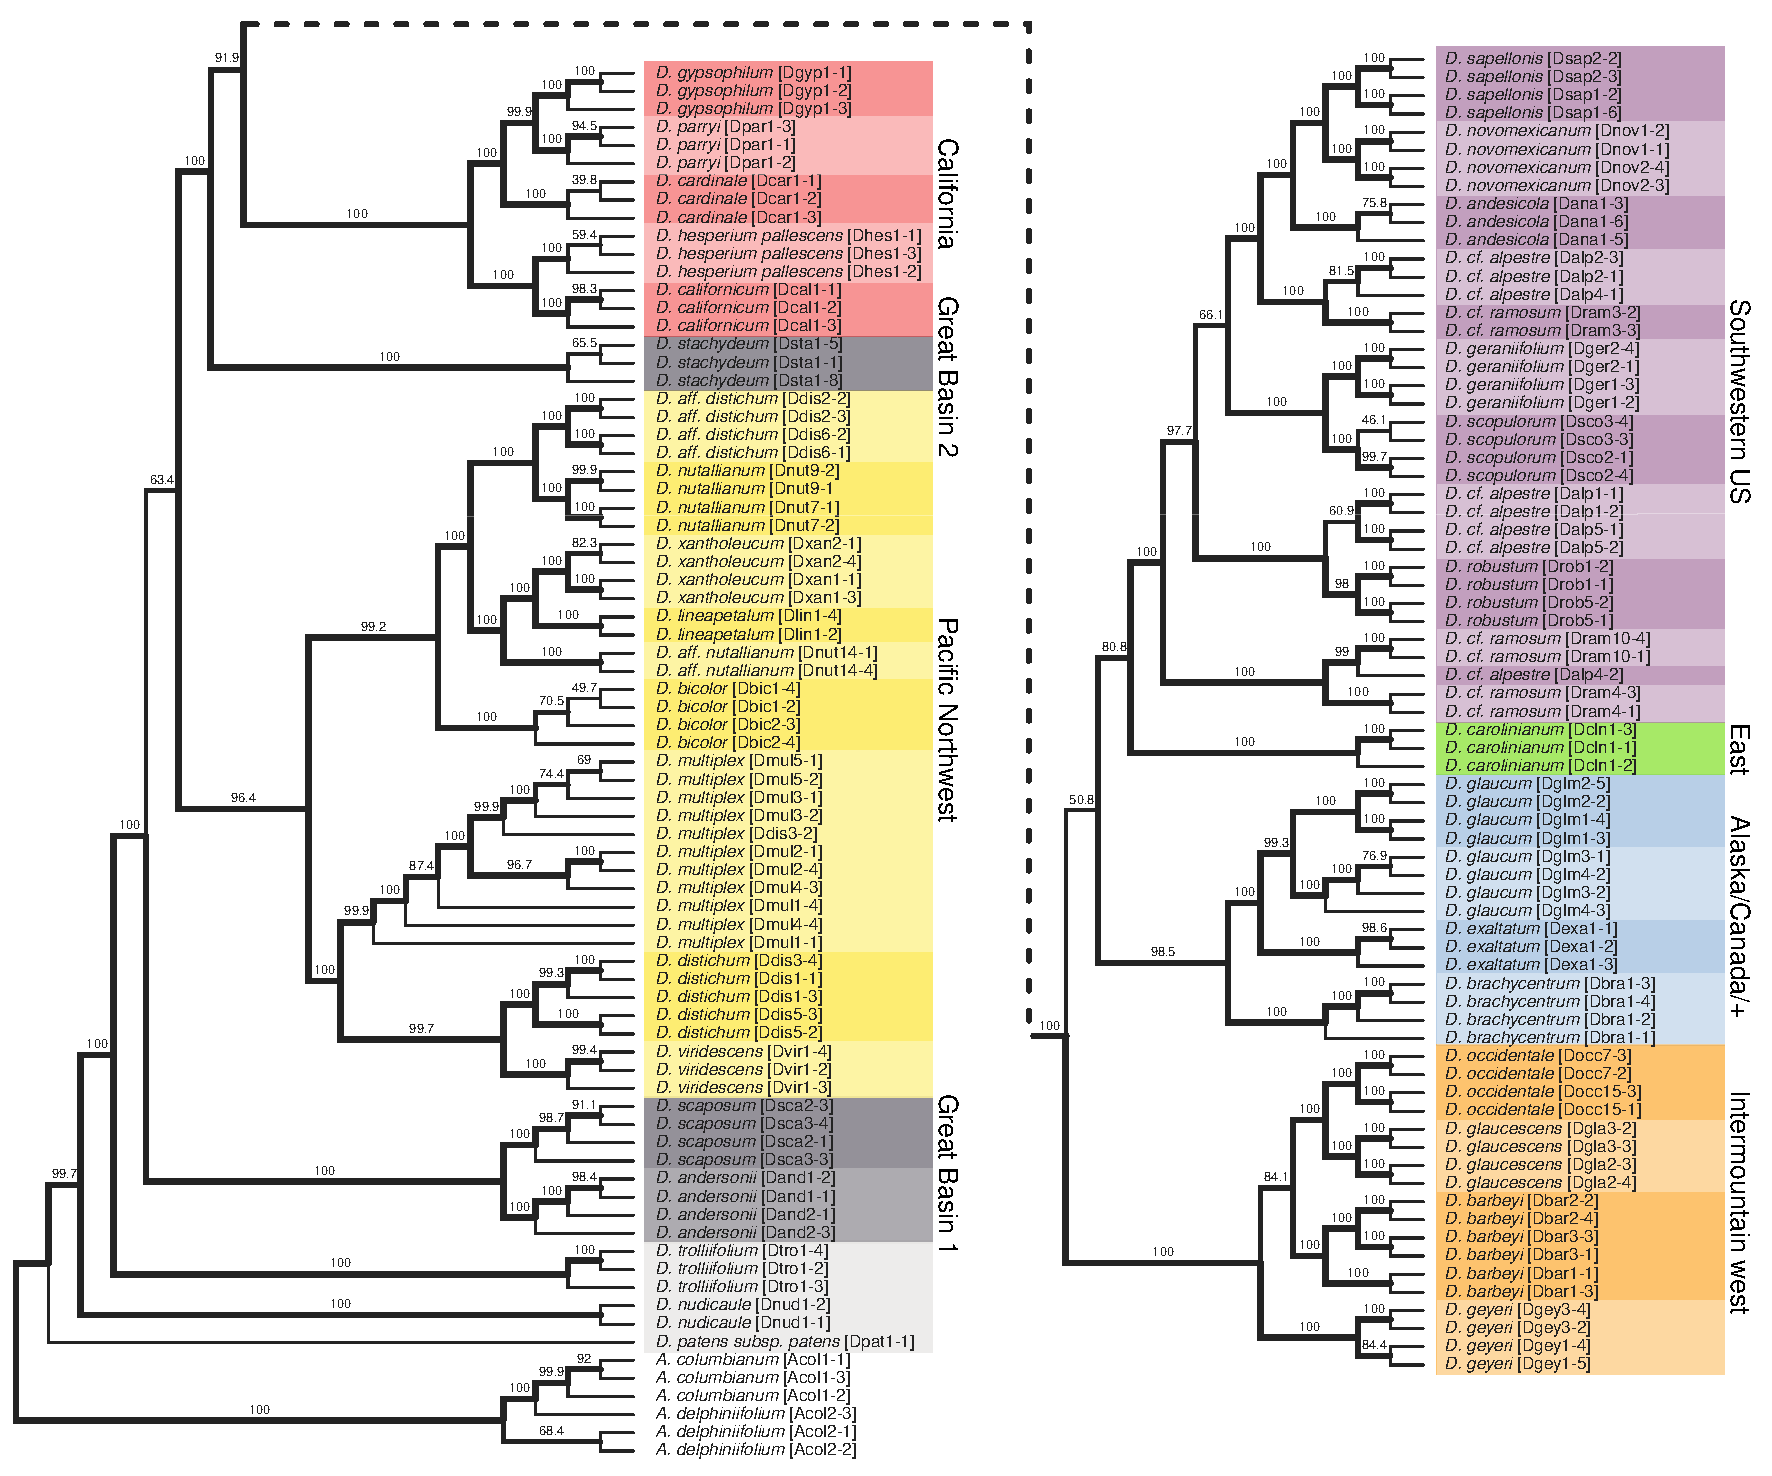
\includegraphics[width=0.99\textwidth]{./figures/caster-trees.pdf}	
	\caption{
		A rooted phylogenetic tree for 150 samples of \emph{Delphinium} sect. \emph{Diedropetala}
		inferred from the min10 SNP dataset using caster-site. Colored rectangles highlight
		groups that correspond well with discrete geographic regions, representing higher-level 
		clades. Replicate samples within each taxon form monophyletic clades, except in the case
		of \emph{D. distichum}, \emph{D. nuttallianum}, \emph{D. cf. ramosum}, and \emph{D. cf. alpestre}.
	}
	\label{fig:bigtree}
\end{figure}


%%%%%%%%%%%%%%%%%%%%%%%%%%%%%%%%%%%%%%%%%%%%%%%%%%%%%%%%%%%%%%%%%%%%%%%%%%%%%%
%%%%%%%%%%%%%%%%%%%%%%%%%%%%%%%%%%%%%%%%%%%%%%%%%%%%%%%%%%%%%%%%%%%%%%%%%%%%%%
%%%%%%%%%%%%%%%%%%%%%%%%%%%%%%%%%%%%%%%%%%%%%%%%%%%%%%%%%%%%%%%%%%%%%%%%%%%%%%
%%%%%%%%%%%%%%%%%%%%%%%%%%%%%%%%%%%%%%%%%%%%%%%%%%%%%%%%%%%%%%%%%%%%%%%%%%%%%%
%%%%%%%%%%%%%%%%%%%%%%%%%%%%%%%%%%%%%%%%%%%%%%%%%%%%%%%%%%%%%%%%%%%%%%%%%%%%%%
\section{Results}
\subsection{Genomic ddRAD sequencing and assembly}
Genomic sequencing yielded a mean of 1,071,118 (+/- S.D. 712,371) raw reads 
across all samples, which were assembled into relatively similar numbers of 
\emph{de novo} clusters within each sample (mean +/- S.D = 19,261 +/- 7,331). 
% 
We dropped samples with fewer than 1000 clusters. 
After clustering across the remaining samples and applying filters, 
the `min4' dataset included 80,169 loci, with the total alignment size of
150 samples x 6,490,732 sites (85.93\% missing) and contained 556,493 
SNPs (68.80\% missing). 
The `min10' dataset included 29,196 loci with a total alignment size of 
150 samples x 2,652,279 sites (70.96\% missing) and contained 399,001 SNPs
(58.03\% missing).


\subsection{Phylogenetic inference recovers monophyletic taxa}
All phylogenetic analyses recovered topologies showing individuals of the same 
species consistently grouped into monophyletic clades, with a few exceptions 
observed within \emph{D. ramosum}, \emph{D. alpestre}, \emph{D. distichum}, and 
\emph{D. nuttallianum} (addressed below in the context of admixture).
% 
Caster-site recovered the same tree topology from both the `min4' and `min10' 
datasets (Fig.~\ref{fig:bigtree}, Fig.~\ref{fig:S1}), while the ML trees
inferred by raxml-ng differed from each other, and from the caster topology.
% 
These differences are concentrated across the backbone of the tree, in the 
order of relationships among several major clades, which generally received
low support across all trees
% These differences are largely due to low backbone support affecting the ordering
% of higher-level relationships across all trees
(Fig.~\ref{fig:S2},~\ref{fig:S3}).
% 
Tree distances, measured using the generalized Robinson-Foulds mutual clustering
information metric \citep[MCI;][]{smith_information_2020}, show that the two
ML topologies share 93.3\% of information in common, while the caster topology
shares 86.0 and 91.3\% of information in common with the ML min4 and min10 
trees, respectively.


A set of higher-level clades was recovered across all trees that shows a strong
concordance with biogeographic regions.
This includes taxa associated with the Great Basin, Pacific Northwest, California, 
Intermountain West, Alaska/Canada, the Southwestern US, and Eastern North America
(Fig.~\ref{fig:sptree}a-b). 
% 
All of our tree hypotheses support three early diverging lineages that split
from the rest of our sampled \emph{Delphinium} taxa early in the radiation. 
This includes \emph{D. patens}, \emph{D. nudicaule}, and \emph{D. trolliifolium},
which are distributed in central California, northern California, and northern 
California and the Pacific Northwest, respectively. We focus most of our further
analyses and discussion on the larger recovered clades in our study.
% 


\begin{figure}[t!]
	\centering
	\includegraphics[width=0.95\textwidth]{./figures/Fig2_sptree.pdf}
	\caption{
		Phylogeny and biogeographic distribution of \emph{Delphinium} sect. \emph{Diedropetala}.
		(a) Locations of samples used in this study.	Color codes match to those used to 
		represent distinct clades in (b) that correspond closely with the following
		biogeographic regions (yellow: Pacific Northwest, red: California, orange: 
		Intermountain West, blue: Alaska and Canada, green: Eastern USA, purple: 
		Southwestern USA, black: Great Basin, grey: other).
		(b) A rooted species tree topology inferred from the min10 SNP dataset using 
		caster-site with population mapping of 150 individuals to 41 populations, 
		shown with local block bootstrap supports.
		One or more biogeographic states occupied by each taxon are shown in a colored
		marker next to each tip.
		The current subsection designation of each taxon from the Flora of North America is
		indicated next to each tip.
		(c-f) There is substantial conflict across the backbone of the tree, which resolved into
		different topologies when analyzed using different datasets or methods.
		Support for monophyly of each clade is consistently >95\% (values at the tips
		of each tree), but support for internal splits between major clades have lower 
		support.
		(g) Images of members of \emph{Delphinium} sect. \emph{Diedropetala} 
		(Photo credits: \emph{D. xantholeucum} from Eastern Washington University, 
		and \emph{D. viridescens} from the Burke Herbarium).
	}
	\label{fig:sptree}
\end{figure}


\subsection{Higher-level clades correspond strongly with biogeographic regions}
We designate eight named clades that were consistently recovered across our
phylogenetic analyses and correspond well to geographic regions. None of these
clades corresponds uniquely with an existing taxonomic subsection in Warnock's
FNA treatment (Fig.~\ref{fig:sptree}b). 
% 
Support for monophyly of each of these clades is >95\% in all trees, despite 
the fact that their ordering varies and has low support among trees
(Fig.~\ref{fig:sptree}c-f).
% 
The grouping of clades IMW, ALCA, ENA, and SW is consistently recovered with 
100\% support, uniting a clade that extends from Alaska to the southern Rocky
Mountains. By contrast, relationships among clades distributed in California 
(CAL) and the Great Basin (GB1 and GB2) are more variable among our trees.
% 
% 
% This may be a result of admixture between species in the CAL clade and other
% early diverged lineages that also occur in California, which we examine below.
% 
% Given the uncertainty in the order of relationships among these higher-level 
% clades, and our incomplete taxon sampling, we are unable to reconstruct 
% it would be premature to draw strong
% conclusions from our results about the order and dynamics of historical biogeography
% in this clade.
% % 
% Nevertheless, our finding of strongly supported clades that correspond to distinct
% biogeographic regions represents a major revision to our understanding of the 
% phylogeny of \emph{Delphinium} sect. Diedropetala, suggesting need for a major 
% taxonomic revision.
% 
% In the following sections, we focus on elucidating the impact of hybrid admixture 
% on our phylogenetic hypotheses.

%%%%%%%%%%%%%%%%%%%%%%%%%%%%%%%%%%%%%%%%%%%% Maybe we save this section for the discussion????
% Consistent clades.
The GB1 clade occurs in the Great Basin, and is represented in our tree
by \emph{D. scaposum} sampled from SE Nevada and NW Arizona, and 
\emph{D. andersonii} sampled from southern Idaho.
% and the populations of \emph{D. andersonii} from southern Idaho. 
 % and includes \emph{D. scaposum} and
% \emph{D. andersonii}. 
% Our sampled populations of \emph{D. scaposum} are from SE Nevada and NW Arizona, 
% and the populations of \emph{D. andersonii} from southern Idaho. 
This clade does not group with the only other taxon we sampled from the Great
Basin, \emph{D. stachydeum}, from northern Nevada. This taxon occurs as the
sole member of its clade, which we designate GB2. 
% 
This split into separate clades aligns with morphological differences between these
two groups, with \textit{D. stachydeum} exhibiting a larger stature, denser 
inflorescences and distinctive fruits when compared to \textit{D. scaposum} and 
\textit{D. andersonii}. 
% 
Neither clade corresponds to an existing taxonomic subsection, and the 
subsection names the taxa are assigned to each appear non-monophyletic on 
our phylogeny.
% Importantly, \emph{D. scaposum} and \emph{D. andersonii} 
% are currently placed in the subsection \textit{Subscaposa} and \emph{D. stachydeum} 
% is placed in the subsection \textit{Wislizenana}, both of which have representatives
% spread across several clades of the phylogeny.

% 
The PNW clade corresponds to taxa distributed in mountainous regions in and around the Columbia
Plateau in E Washington, NE Oregon, Idaho, and W Montana. It includes \emph{D. lineapetalum}, 
\emph{D. xantholeucum}, \emph{D. nuttallianum}, \emph{D. distichum}, \emph{D. bicolor}, 
\emph{D. viridescens}, and \emph{D. multiplex}. We recover both \emph{D. nuttallianum}
and \emph{D. distichum} as polyphyletic, possibly as a result of admixture, which we
investigate below. 
Morphologically, this clade contains several species of short‑stature that have basal
leaves and small to moderate inflorescences (3-30 flowers), but which vary in sepal
color, spur length, and seed morphology.
% 
The seven taxa in this clade are grouped into five different subsections in the 
current FNA treatment, suggesting that our results represent a major departure from
their expected relationships based on morphology.

% 
The CAL clade includes taxa distributed primarily in California, represented in our
tree by \emph{D. californicum}, \emph{D. hesperium}, \emph{D. cardinale}, 
\emph{D. gypsophilum}, and \emph{D. parryi}. 
These five taxa, which are 100\% supported as monophyletic both within species 
and as a group in our phylogenetic analyses, are currently placed in four different 
subsections in the current FNA treatment. These species tend to have tall stems, 
long spurs, an absence of winged seeds, and exhibit a range of flower color
variation.


The IMW clade corresponds to taxa distributed in the Intermountain West region 
between the Cascades/Sierra Nevada and the Rocky Mountains.
It is represented by four species in our study, 
\emph{D. geyeri}, \emph{D. barbeyi}, \emph{D. occidentale}, and \emph{D. glaucescens}.
Several of these species have large geographic ranges spanning this region, 
in subalpine high‑elevation environments.
% 
They all share a medium stature with moderate sized inflorescences of blue-purple flowers 
with medium length (9-18 mm) spurs. 

% Jared add info about lack of eastern species samples; missing clade here essentially 
The ALCA clade corresponds primarily to \emph{D. brachycentrum}, which is endemic to 
tundra environments in Alaska and northern Asia, and \emph{D. glaucum}, a tall larkspur 
whose range spans much of the North American Cordillera from Alaska and British Columbia 
down through the Northern Rockies, with populations also present in the Cascades and Sierra Nevada. 
Surprisingly, this group also includes \emph{D. exaltatum}, which occurs broadly in eastern North
America. The two populations of \emph{D. glaucum} group monophyletically in the caster topologies, 
but \emph{D. glaucum} from Alaska groups with the \emph{D. brachycentrum} in the ML topologies.
% Members of this are all in the Exaltata subsection,
% representing the "tall larkspurs". 
Members of this clade vary in stature (the subarctic \emph{D. brachycentrum} is short) 
but are united by having glabrous to glaucous stems, moderate‑length spurs, 
paler flowers, and tending to occur in moist and rocky habitats, in contrast to 
morphologically similar, but dry adapted members of the CAL clade.


The SW clade is represented by eight taxa in our study which share a biogeographical
distribution throughout the southwestern United States. This includes
\emph{D. scopulorum}, \emph{D. geraniifolium}, \emph{D. alpestre},
\emph{D. robustum}, \emph{D. ramosum}, \emph{D. andesicola}, \emph{D. sapellonis},
and \emph{D. novomexicanum}. Notably, \emph{D. ramosum} and \emph{D. alpestre}
are both polyphyletic. We recover three separate clades of \emph{D. alpestre}, each
appearing sister to a clade of \emph{D. ramosum}, or of the very morphologically
similar \emph{D. robustum}. We investigate this "replicated divergence" pattern in 
greater detail below. This group is united by all taxa having tall stature, 
large leaves and large inflorescences.


%%%%%%%%%%%%%%%%%%%%%%%%%%%%%%%%%%%%%%%%%%%%%%%%%%%%%%%%%%%%%%%%%%%%%%%%%%%%%%%%%%%%%%%%
%%%%%%%%%%%%%%%%%%%%%%%%%%%%%%%%%%%%%%%%%%%%%%%%%%%%%%%%%%%%%%%%%%%%%%%%%%%%%%%%%%%%%%%%
%%%%%%%%%%%%%%%%%%%%%%%%%%%%%%%%%%%%%%%%%%%%%%%%%%%%%%%%%%%%%%%%%%%%%%%%%%%%%%%%%%%%%%%%

\subsection{Hybridization and Introgression}
Many \emph{Delphinium} species overlap in both geography and phenology in 
western North America, where many putative hybrids have been described.
% 
Results of our f-branch analyses confirm that genomic admixture is widespread
and common both within and between the major clades of \emph{Delphinium} that
we identified (Fig.~\ref{fig:fbranch}).
Admixture is most common between taxa within the same geographically structured
clades, or between clades with overlapping geographic ranges.
% 
These patterns are consistent across alternative species tree hypotheses as well 
(Fig.~\ref{fig:S4},~\ref{fig:S5}).
% 
We suspect that some of these hypothetical introgression events may
represent false positives that can arise from non-independent signals of
admixture among multiple hybridizing taxa \citep{eaton_historical_2015}.
Extinct and unsampled lineages may also contribute to these patterns.
% 
To avoid over-interpretation of these results, we focus below on describing 
the strongest signals of admixture, their taxonomic and geographic scope, 
and whether hybrids have been previously reported for the selected taxa 
based on observational or experimental evidence summarized in the FNA or 
Jepson Manual treatments of \emph{Delphinium}.

\begin{figure}[t!]
	\centering
	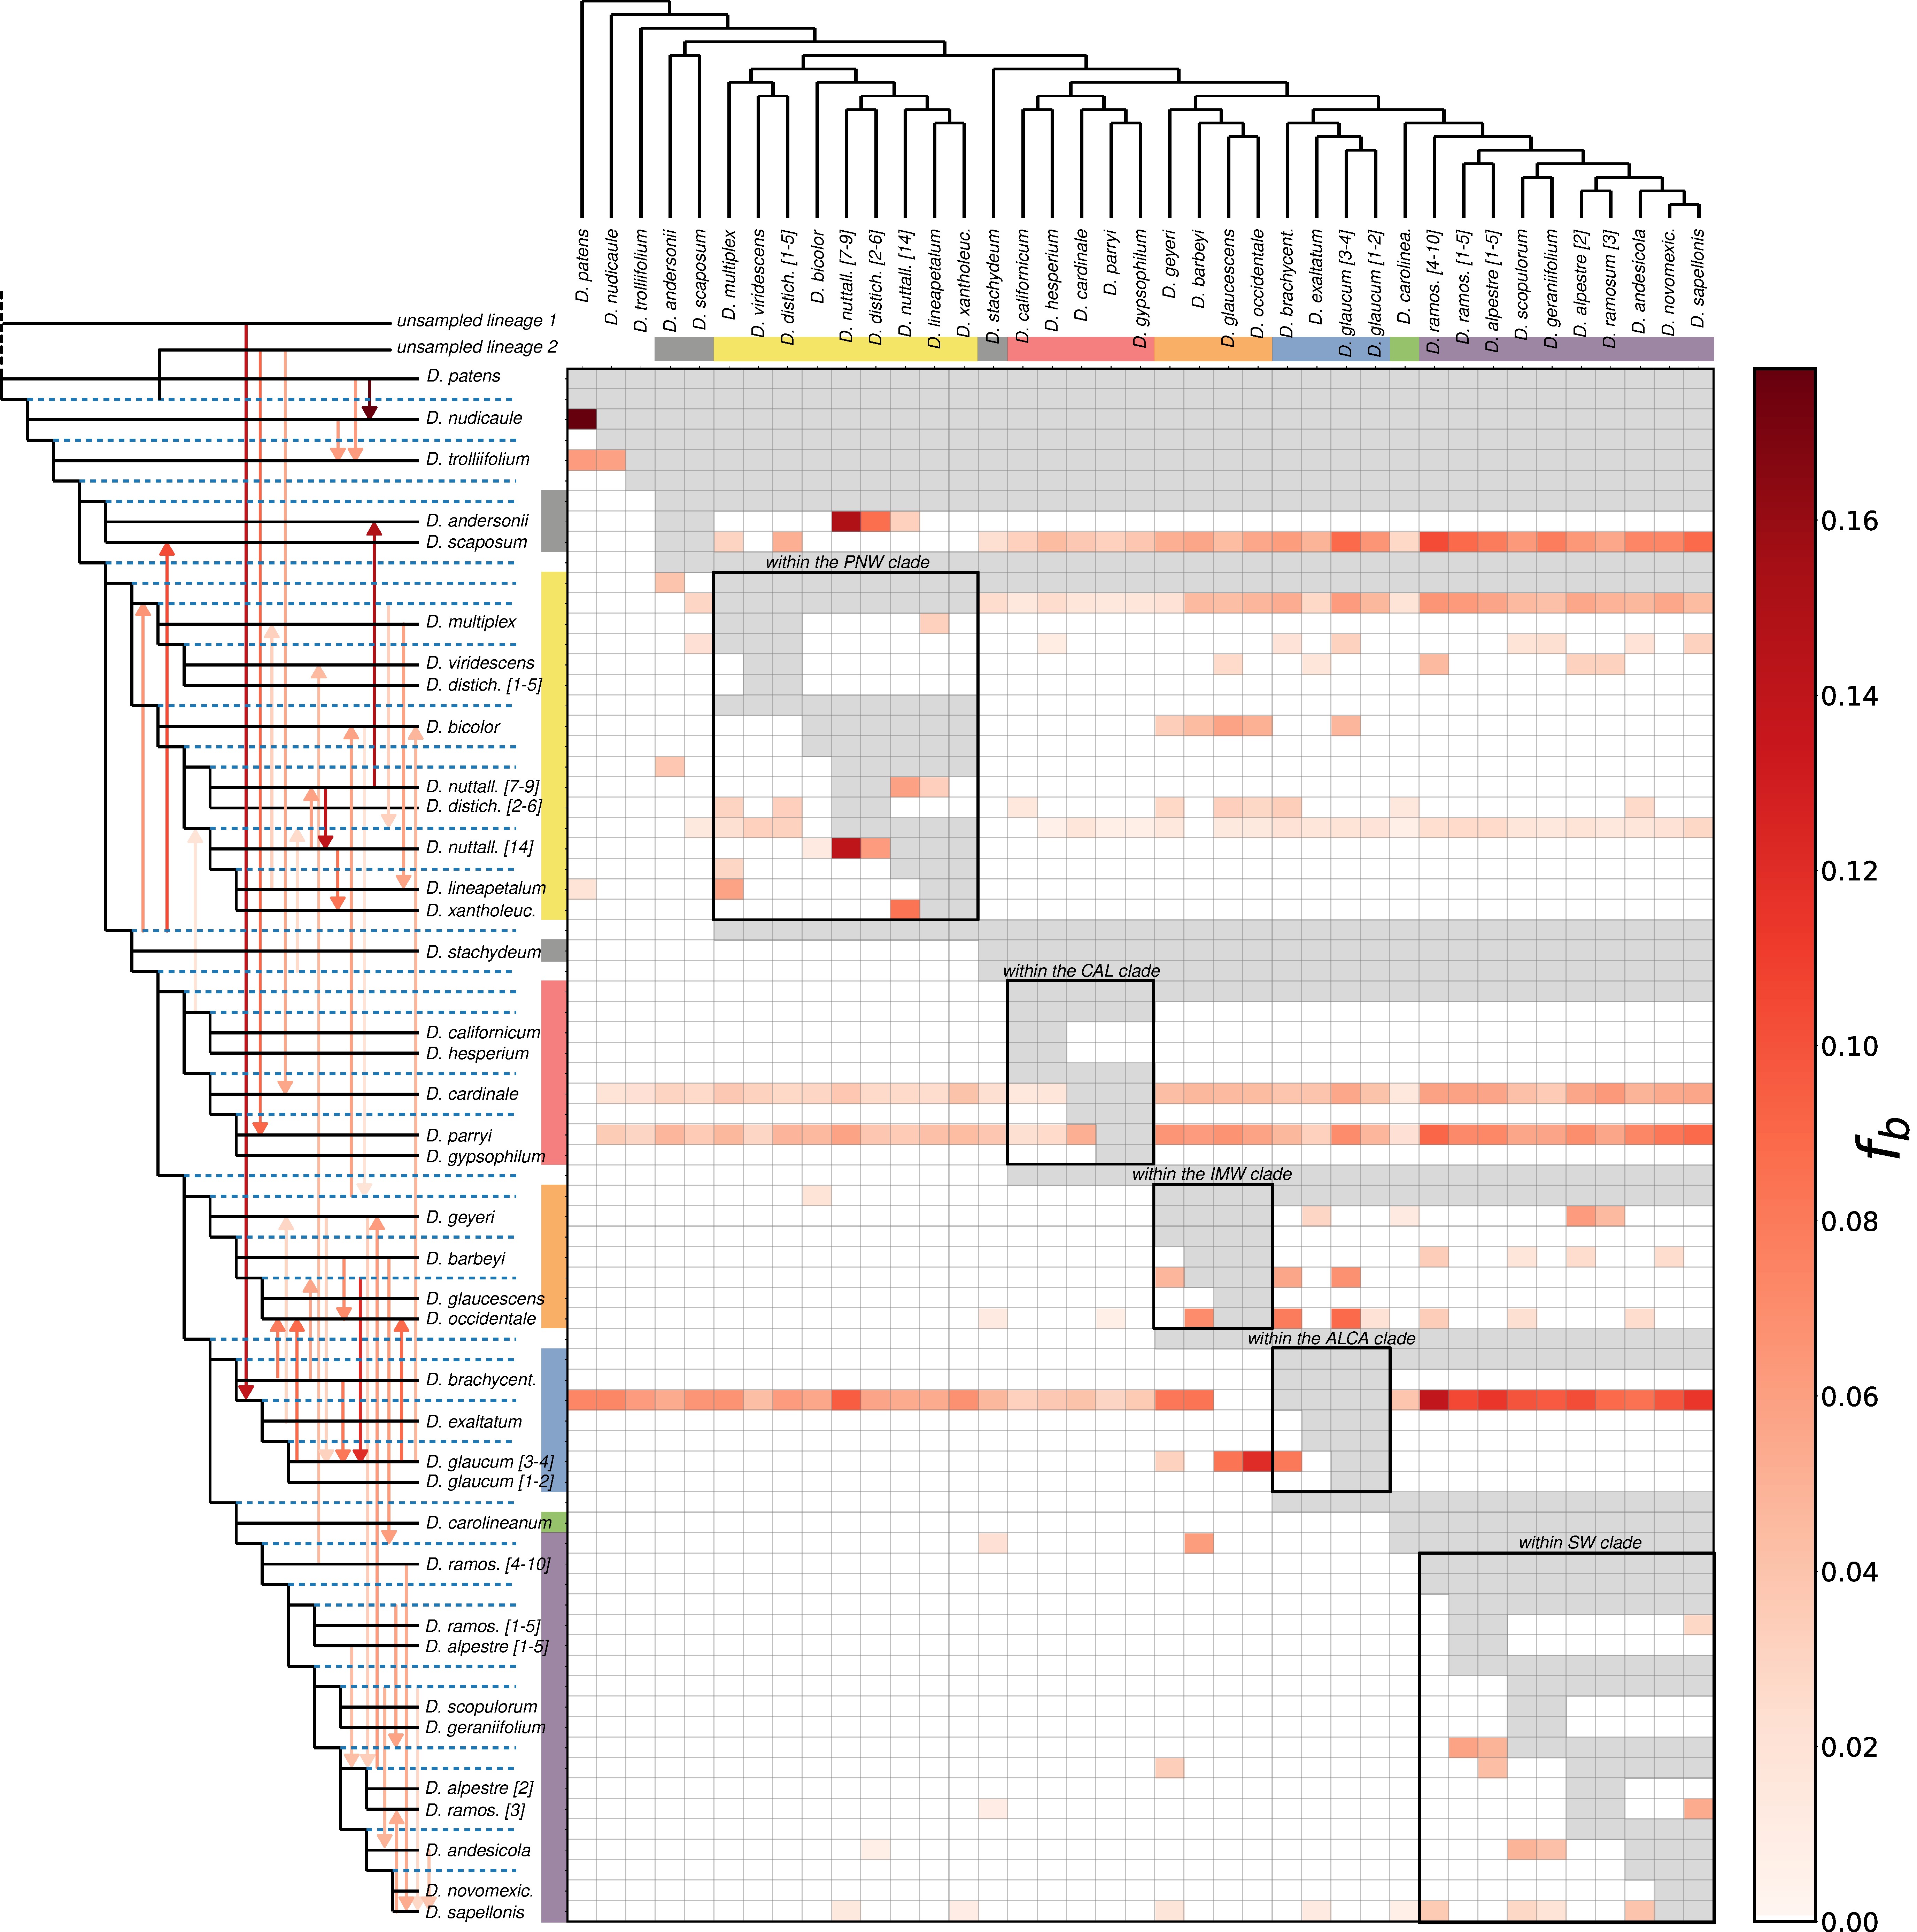
\includegraphics[width=0.95\textwidth]{./figures/fbranch-caster-min10.pdf}
	\caption{
        Genomic admixture proportions between populations of \emph{Delphinium} 
        section Diedropetala estimated using f-branch statistic. 
	}
	\label{fig:fbranch}
\end{figure}

\subsubsection{Early diverged and unsampled lineages}
The strongest signal of admixture is observed in the early diverged lineages 
represented by several taxa co-distributed in California.
The estimated admixture proportion between \emph{D. patens} and 
\emph{D. nudicaule} is approximately 17\%, while admixture between both of 
these taxa and \emph{D. trolliifolium} is approximately 6\%.
% ... while that between x and y and y and z is ...
Given their positions in the tree we cannot distinguish the directionality.
These results are consistent across multiple replicate sampled individuals
in both \emph{D. nudicaule} and \emph{D. trolliifolium}, lending increased
confidence, although we have only one representative of \emph{D. patens}. 
% 
Genomic evidence of admixture between these species is consistent with 
reported observations that both species can hybridize with \emph{D. nudicaule}.
% 
We do not find further evidence of \emph{D. nudicaule} hybridizing with other
taxa in our dataset, despite reports of putative hybridization with 
\emph{D. andersonii} and \emph{D. nuttallianum}.
% 

Although none of these early diverged lineages is supported as a unique introgressive
donor into other \emph{Delphinium} taxa in our study, they do potentially provide 
evidence of other \emph{unsampled} (or ghost) lineages that may be introgressive donors.
This is most notable in the clade sister to \emph{D. brachycentrum}, which includes 
the widespread taxa \emph{D. glaucum} and \emph{D. exaltatum}. 
This clade has the odd result of appearing admixed with every other sample in our 
phylogeny.
Our best hypothesis to explain this involves introgression from a divergent unsampled
lineage which we designate "unsampled lineage 1" (Fig.~\ref{fig:fbranch}). 
% 
\emph{D. brachycentrum}, which lacks this signal of admixture, is the lone taxa in our
study that also occurs in Asia. If it only recently dispersed to North America, that 
could explain why this introgression event only occurred into other North American 
members of this clade.
% 
An additional ancient introgression event may have occurred into the CAL clade, 
involving \emph{D. cardinale} and/or \emph{D. parryi}, from an unsampled lineage we 
designate "unsampled lineage 2". Because this admixture signal is observed with respect 
to all taxa except \emph{D. patens}, we propose that it may be derived from an unsampled 
or ghost member of a clade that diverged between \emph{D. patens} and \emph{D. nudicaule}, 
and which like them, exists or existed in California. 


\subsubsection{Admixture between geographic clades}
% 
In addition to the early diverged lineages which overlap in California, there is
also evidence of introgression between several other major biogeographic
clades, particularly among members whose ranges overlap.
% 
This includes introgression between GB1 and PNW, involving \emph{D. aff. nuttallianum}
from N Utah and \emph{D. andersonii} from S Idaho. These taxa are reported to 
hybridize [CITE Jepson], and our analyses suggest that introgression is largely 
unidirectional into \emph{D. andersonii}.
% 
The widespread taxon \emph{D. glaucum} also appears admixed with several lineages, 
consistent with reports that it forms many types of hybrids.
Our genomic results confirm introgression with its close relative \emph{D. brachycentrum}, 
as well as with \emph{D. occidentale} from the IMW clade. 
The latter has been described as a hybrid between \emph{D. glaucum} and the 
IMW taxon \emph{D. barbeyi}. Although \emph{D. occidentale} appears admixed with both
species, it also shares affinity with \emph{D. glaucescens} and perhaps additional 
admixture with other taxa. Thus, our results suggest \emph{D. occidentale} has a more 
complex origin that deserves further investigation.
% 
Another taxon that appear admixed with \emph{D. glaucum} is \emph{D. bicolor},
a widespread taxon from the PNW clade, which has not been previously reported. 
We do not observe admixture between \emph{D. glaucum} and \emph{D. stachydeum} 
from the GB2 clade, despite reports of hybrids between these taxa.
% 

Further evidence of introgression between divergent clades is observed between
members of the SW clade and members of both PNW and IMW, but none of these 
admixture proportions is particularly high.
% 
Although our f-branch results appear to support frequent admixture between divergent
biogeographic clades, this pattern is largely driven by a few widespread species that
hybridize abundantly, notably: \emph{D. nuttallianum} (PNW clade); 
\emph{D. barbeyi} (IMW clade); 
and \emph{D. glaucum} (ALCA clade). 
% 
The ENA and CAL clades are relatively isolated from these widespread taxa, both 
geographically and ecologically, and are conspicuously absent of across-lineage
introgression from these frequently hybridizing taxa.

% Dnut-14 is real.
% Ddis-15 is real.
Based on inferred patterns of introgression we are better able to interpret 
potential taxonomic implications of our phylogenetic results.
Our populations of \emph{D. aff. nuttallianum} (7-9) which appear highly admixed
between 


\subsubsection{Admixture within geographic clades}

There is also abundant evidence of admixture between species within each 
biogeographic clade.
% 
For example, within the PNW clade nearly every taxon is admixed with either 
\emph{D. multiplex} or \emph{D. aff. nuttallianum}; in the IMW clade most taxa
are admixed with \emph{D. barbeyi}; and in the SW clade there is a low level of
admixture between most lineages.
% 
Given that these same taxa are widely involved in introgression between the
biogeographic clades, this suggests that alleles from nearly any species are
capable of being introgressed into another.
% 
An exception is the CAL clade, shows little evidence of introgression between 
close relatives. 
This clade is notably characterized by high variation in flower color, 
suggesting that reproductive divergence may play an important role in 
reducing interspecies gene flow in this clade.




\begin{figure}[t!]
	\centering
	  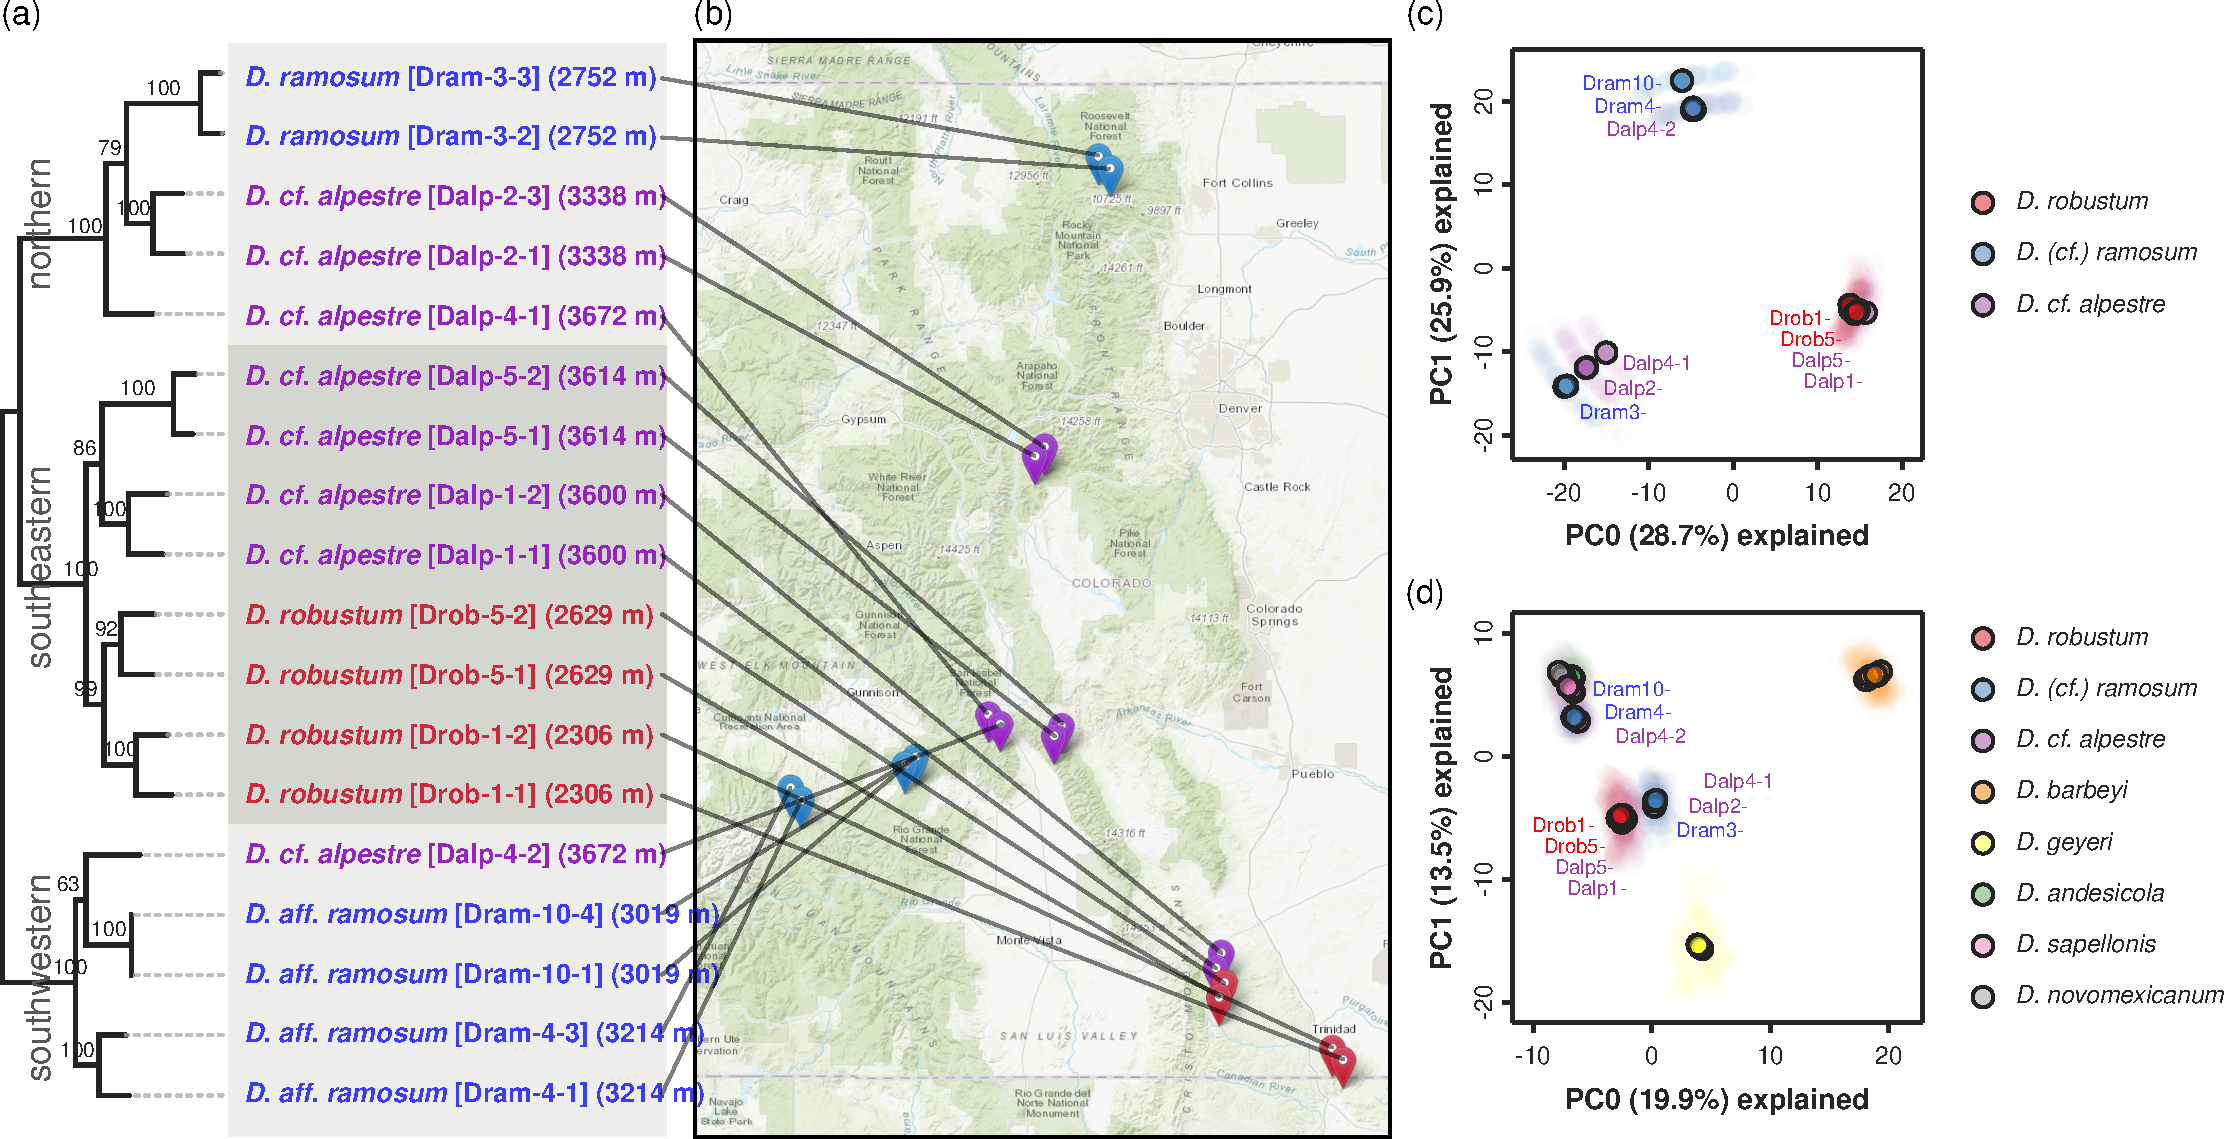
\includegraphics[width=0.99\textwidth]{./figures/ramosum-robustum-alpestre3}	
	\caption{
        Hybrid complex of \emph{D. robustum}, \emph{D. ramosum}, and \emph{D. cf. alpestre} in the Southern Rocky Mountains. 
        (a-b) Three distinct clades are consistently supported in our phylogenetic analyses, which corresponding more closely with geography than with species determinations based on morphology.
        (c-d) Phylogenetic analyses focused on the subset of samples in this complex
        recovers the same three clades, with similar topologies recovered by caster-site and raxml-ng, respectively.
        (e-f) PCA of the subset of samples in this hybrid complex.
        (g-h) PCA with the inclusion of \emph{D. sapellonis}, which shows evidence of admixture.        
	}
	\label{fig:robustum}
\end{figure}


\subsubsection{Replicated Divergence in the \emph{D. ramosum} complex}
% 
There is substantial disagreement across floras concerning the distinction between 
\emph{D. ramosum}, \emph{D. robustum}, and \emph{D. alpestre} 
\citep{ewan_synopsis_1945,ackerfield_flora_2022,weber_},
a complex of species native to Colorado and New Mexico that are grouped into
our SW clade.
% 
Our dataset includes multiple sampled populations of each species. 
% 
In phylogenetic analyses using our full dataset both \emph{D. ramosum} and 
\emph{D. alpestre} are polyphyletic, with the high elevation \emph{D. alpestre}
resolved into three different clades (Fig.~\ref{fig:bigtree}).
We refer to each of these populations exhibiting the distinct high elevation 
diminutive phenotype as \emph{D. cf. alpestre}.
Similarly, we use the designations \emph{D. ramosum} and \emph{D. robustum} for
the two populations exhibiting the lower elevation phenotype in the corresponding 
geographic region where their types were originally described. 
The final ramosum-like population, from the southwestern San Juan Mountains, 
we refer to as \emph{D. aff. ramosum}
% 
Using a more dense subsampled sequence alignment generated for this clade,
comprising X x X Mbp with X\% missing data, we inferred an additional ML 
concatenation tree which further confirmed the phylogenetic relationships
observed in the larger tree (Fig.~\ref{fig:robustum}a).
% 
As with the broader phylogenetic patterns in \emph{Delphinium}, relationships
among populations within this clade match closely with geography.
%  
% Within each region, the population of \emph{D. alpestre} occurs at higher 
% elevations, consistent with its more diminutive stature, suggesting that this
% taxon may represent either high-elevation plasticity, or replicated adaptations
% to high elevations.

% 
We also examined patterns of ancestry among these populations using PCA performed
on 2068 unlinked SNPs from the 18 samples in this species complex.
Similar to our phylogenetic results, this clearly groups samples into three
clusters corresponding to the phylogenetic clades (Fig.~\ref{fig:robustum}c)
% 
However, when we add additional taxa representing other SW clade taxa, and
putative admixed taxa from the IMW clade, 
we find evidence that their relationships are shaped by admixture.
% 
This PCA analysis was performed on 1792 unlinked SNPs across 39 samples 
from 8 taxa (Fig.~\ref{fig:robustum}d). 
Here, the southeastern and southwestern clades from this complex both 
group closer to \emph{D. geyeri} than do samples from the northern 
clade, which groups more closely with other SW clade taxa. 
% 
While this suggests admixture may contribute to the phylogenetic patterns,
it does not explain the replicated pattern of morphological divergence 
between \emph{D. cf. alpestre} and its closest relative within each subclade.
Further work is needed to investigate the role of plasticity versus 
replicated adaptation in driving this pattern.



\section{Discussion}

\subsection{Phylogeny and Higher-level Taxonomy in \emph{Delphinium} sect. \emph{Diedropetala}}
% summarize broad results: New phylogeny with 8 geo clades and abundant admixture
We generated a large-scale genomic ddRAD-seq dataset to resolve phylogenetic 
relationships among populations and species spanning 34 taxa in the North American 
clade \emph{Delphinium} sect. \emph{Diedropetala}.
% 
Our phylogenetic results recovered most populations within taxa as monophyletic, 
and grouped all taxa into eight consistently recovered higher-level clades 
that are strongly associated with biogeographic regions.
% 
We applied a range of phylogenetic methods, and data filtering approaches,
to examine potential impacts of missing data or methodological biases.
% 
The primary disagreement among these results involves the order in which the
eight major clades diverged across the backbone of the tree. These relationships
received low support across all trees.
% 
This is consistent with the results of f-branch statistics which indicate abundant
hybrid introgression between species both within and between many of these clades.
% 
Our new phylogenetic hypotheses for the relationships within 
\emph{Delphinium} sect. \emph{Diedropetala} present a significant advance for 
understanding the history of this North American plant clade. 
Most significantly, our results highlight the dominant role of geography and 
hybrid admixture in shaping their diversification.


% how does this relate to existing classifications
Our phylogenetic results conflict with existing higher-level taxonomy in 
\emph{Delphinium} sect. \emph{Diedropetala}, including the current FNA treatment,
which groups many taxa on the basis of morphological variation in leaf, flower, 
and root variation.
% 
Although our study does not include complete taxon sampling, we have
included at least one representative of each subsection in the FNA treatment, 
allowing us to assess the concordance between molecular versus morphological 
similarities.
% 
Eight out of nine of the subsections in the FNA are recovered as polyphyletic
in our phylogenies, representing discordance for every subsection for which
we have more than one sample.
This highlights the need for an updated taxonomy for this clade in light of 
genomic evidence.
% 
We propose a new taxonomic treatment in which the eight biogeographic clades 
in our study are designated as named subsections. Based on existing taxon 
descriptions in the FNA, we describe the characters that unite members in each
of these subsections, and provide a dichotomous key 
(Supplemental Materials).


% SYNGAMEON---
\subsection{The Western North American \emph{Delphinium} Syngameon}

- we detect abundant hybrid introgression across the clade.
- this is consistent with many previous descriptions of hybrids.
- many references.
- genomic data is important for understanding the consequences of 
  both historical and ongoing hybridization in terms of genomic
  introgression between lineages.


- the extent of introgression across the clade raises the question
  of whether phylogenetic results represent historical patterns of
  populations splitting across barriers, versus more recent patterns
  of gene flow that may overwrite past patterns.
- additional analyses are need to further investigate these questions.
- here, we were are somewhat limited by the information available in
  de novo assembled RAD-seq data. Moreover, the short lengths of our
  reads increase the challenge of distinguishing paralogs, and reduce
  our ability to infer individual gene trees for each locus, and apply
  gene tree based inference methods.
- One such method that needs further exploration is network inference,
  which we could not apply here. This could help with resolving the order
  of divergence across the backbone of the tree.
- This, along with additional sampling of taxa, will be important towards
  reconstructing the biogeographic history of the clade, and their order
  and timing of dispersal between these regions.


- the term syngameon is used to describe this type of pattern.
- this has been observed in lineages like X, Y and Z.
- this is emerging as a pattern in WNE.
- in delphinium it seems that several super-hybridizers may play
  a major role in spreading alleles between lineages.
- this could allows for local adaptation to occur repeatedly.



There is also abundant evidence of admixture between species within each 
biogeographic clade, which raises the question of whether their grouping 
is a consequence of localized gene flow.
% 
For example, within the PNW clade nearly every taxon is admixed
with either \emph{D. multiplex} or \emph{D. aff. nuttallianum}; 
in the IMW clade most taxa are admixed with \emph{D. barbeyi}, and in the 
SW clade there is a low level of admixture between most lineages. 
Given that many of these taxa are also involved in across-clade introgression, 
there is a high potential for alleles from nearly any taxon to be exchanged
with another.
% 
Given the young age of the \emph{Delphinium} sect. Diedropetala clade, it 
is possible and the local differences between taxa may reflect local 
adaptation from a shared gene pool more 
% 
Within most of the major biogeographic clades we find evidence of introgression
between closely related species, which raises the question of whether their 
grouping into a clade truly reflects a history of dispersal and divergence, or
is a consequence of gene flow 
% 
Whether this is true of the other biogeographic clades is less clear. 
% 
Within the PNW clade the strongest signature of introgression occurs between the
two lineages of \emph{D. nuttallianum}. 



% Morphological variation/convergence
\emph{D. californicum} can be easily confused with \emph{D. glaucum} or \emph{D. exaltatum}, and
is most readily distinguished by its western distribution and earlier flowering time [CITE FNA]. 
It is, however, quite distantly related in our results.

Add a couple sentences about tall larkspurs being longer-lived vs. shorter-lived perennials and how that trait maps onto the tree pretty well.
Biogeography hypothesis; asia - north america disjunctions; what else dispersed to NA at this time? Other plant genera that might support this hypothesis of glacial extirpation and then migration from south to north?


\subsection{Replicated Adaptation or Cryptic Speciation}
% OCCIDENTALE HYBRID?
Importantly, our collections and analyses help to resolve long-standing disagreements 
concerning the taxonomy of multiple species. For example, we included multiple samples
of \emph{D. occidentale}, a species recognized by Ewan (1945) and Holmgren (2012), 
but which Warnock (1997) describes as a hybrid between \emph{D. glaucum} and 
\emph{D. barbeyi}. 
% 
Our replicate population sampling, multiple phylogenomic analyses, and admixture 
analyses together provide multiple lines of evidence for interpreting the distinctiveness
of this taxon. Our results show that \emph{D. occidentale} is admixed \emph{D. glaucum} 
and \emph{D. barbeyi}, but also shares many alleles with \emph{D. glaucescens}, suggesting
that this taxon also plays a role in its history. Given that nearly all taxa in our 
study show some evidence of admixture, we propose that \emph{D. occidentale} 
may be just as deserving as any other taxon of species status.


% RAMOSUM COMPLEX
A similar case is observed in the \emph{Delphinium ramosum} complex underscores the possibility that Delphinium alpestre is not a single taxon, but rather two separate taxa that independently speciated into alpine environments following the split of a progenitor population of Delphinium ramosum or robustum. Considering that these taxa belong to the most recently diverged clade of Delphinium sect. Diedropetala, future research involving these species may be a fruitful avenue for studies involving convergent plant adaptation in mountain environments.

Thus, although each distinct geographic clade in the species complex formed by 
\emph{D. robustum}, \emph{D. ramosum}, and \emph{D. alpestre} varies in its
proportion of admixture with other species, the populations of \emph{D. alpestre}
are not very genetically distinct from 

these clades retain two distinct
morphological types distributed with respect to elevation, but which do not
appear to be genetically distinct. 
% 


\subsection{Conclusions}
Our phylogenomic analyses present new hypotheses and insights into the evolutionary
history of this rapidly radiated clade, and demonstrate that the divergence history
of this group is more complex than morphology alone reveals. 
% 
We discover that an overwhelming signal of geographically structured ancestry, 
where species co-distributed in connected 

Future work should include the remaining unsampled taxa so that questions concerning biogeographic history, dispersal, and diversification linked to climatic, topographical, or pollination shifts (Sharma et al., 2024) s=ince Delphinium’s arrival to North America can be tested. While a full sampling of all Delphinium sect. Diedropetala species is required, the need for a major revision of higher-level taxonomy within this clade is clear, which should aim to identify morphological characteristics among species that are concordant with the monophyletic clades supported by molecular evidence.


\bibliographystyle{ecol_let}
\bibliography{references}  



\beginsupplement

\begin{figure}[p]
	\centering
	% \includegraphics[width=0.95\textwidth]{./figures/Fig2_sptree.pdf}
	\caption{
		A rooted phylogenetic tree for 150 samples of \emph{Delphinium} sect. \emph{Diedropetala}
		inferred from the min4 SNP dataset using caster-site, with supports shown from
		1000 local block bootstrap replicates. 
		Colored rectangles highlight
		groups that correspond well with discrete geographic regions, representing higher-level 
		clades. Replicate samples within each taxon form monophyletic clades, except in the case
		of \emph{D. distichum}, \emph{D. nuttallianum}, \emph{D. rasomum}, and \emph{D. alpestre}.
	}
	\label{fig:S1}
\end{figure}

\begin{figure}[p]
	\centering
	% \includegraphics[width=0.95\textwidth]{./figures/Fig2_sptree.pdf}
	\caption{
		A rooted phylogenetic tree for 150 samples of \emph{Delphinium} sect. \emph{Diedropetala}
		inferred from the min4 sequence alignment using raxml-ng, with supports shown from
		200 non-parametric bootstrap replicates. 
		Colored rectangles highlight
		groups that correspond well with discrete geographic regions, representing higher-level 
		clades. Replicate samples within each taxon form monophyletic clades, except in the case
		of \emph{D. distichum}, \emph{D. nuttallianum}, \emph{D. rasomum}, and \emph{D. alpestre}.
	}
	\label{fig:S2}
\end{figure}

\begin{figure}[p]
	\centering
	% \includegraphics[width=0.95\textwidth]{./figures/Fig2_sptree.pdf}
	\caption{
		A rooted phylogenetic tree for 150 samples of \emph{Delphinium} sect. \emph{Diedropetala}
		inferred from the min10 sequence alignment using raxml-ng, with supports shown from
		200 non-parametric bootstrap replicates. 
		Colored rectangles highlight
		groups that correspond well with discrete geographic regions, representing higher-level 
		clades. Replicate samples within each taxon form monophyletic clades, except in the case
		of \emph{D. distichum}, \emph{D. nuttallianum}, \emph{D. rasomum}, and \emph{D. alpestre}.
	}
	\label{fig:S3}
\end{figure}


\begin{figure}[p]
	\centering
	% \includegraphics[width=0.95\textwidth]{./figures/Fig2_sptree.pdf}
	\caption{
		f-branch analysis of admixture performed on the raxml-min4 species tree hypothesis.	
	}
	\label{fig:S4}
\end{figure}

\begin{figure}[p]
	\centering
	% \includegraphics[width=0.95\textwidth]{./figures/Fig2_sptree.pdf}
	\caption{
		f-branch analysis of admixture performed on the raxml-min10 species tree hypothesis.
	}
	\label{fig:S5}
\end{figure}



\end{document}



